\section{Trained judges: matched LoRA fine-tuning with four objectives}
\label{sec:lora}

% Provenance: experiments 24, 25 (HelpSteer2) and 29 (ChaosNLI, DICES, HelpSteer2; 1,401 of 1,401 runs verified).
Calibrating a frozen judge changes only its output map.
To test whether the objective also changes what the judge learns, experiments 24, 25 and 29 fine-tune the weights.
We adapt Qwen3-4B-Instruct-2507 and Llama-3.1-8B-Instruct with LoRA~\citep{hu2022lora} (rank 8, $\alpha=16$, top four transformer blocks, plus a rating read-out) on human ratings of HelpSteer2 helpfulness~\citep{wang2024helpsteer2} (five ordinal levels, 1{,}038 held-out responses from 519 held-out prompts), ChaosNLI, DICES and the two-class alphaNLI.
We train four objectives: CE, RPS, mean squared error on the expected rating, and Pearson correlation.
Model, prompt, optimizer (AdamW), three learning rates, mini-batch schedule and validation-RPS selection among four checkpoints are identical across them.
A raw forecast is the network's output.
A calibrated forecast adds a one-dimensional score calibration (1D) or a $(K+2)$-parameter logit calibration fitted on separate ratings, identically for every objective.
Intervals are simultaneous maximum-$t$ 95\% cluster-bootstrap bands over held-out clusters with 4{,}000 draws, both conditional on the matched training draws and crossed with them (draw by held-out unit).

\begin{figure*}[t]
\centering
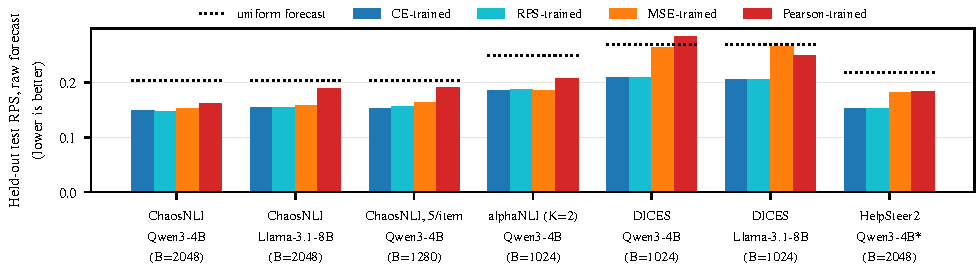
\includegraphics[width=\textwidth]{figures/fig_exp29_four_objectives.pdf}
\caption{\textbf{Pearson-trained judges have higher raw ranked probability score (RPS) than CE-trained judges in all seven setups at the largest budget.}
Four training objectives for LoRA judges at the largest budget, raw forecast.
Vertical axis: held-out test RPS of the network's own forecast, with no post-hoc calibration (0--1; lower is better); the dotted line is the uniform forecast.
Blue: CE-trained; cyan: RPS-trained; orange: MSE-trained; red: Pearson-trained.
Horizontal axis: dataset, base model and development budget $B$ in ratings (one per item unless ``5/item''); half of $B$ trains the weights, and a quarter each selects the checkpoint and fits the calibration.
Test data: held-out items or prompts of ChaosNLI, DICES and HelpSteer2 ($K=2$ for alphaNLI, 3 for ChaosNLI and DICES, 5 for HelpSteer2).
Each judge is the checkpoint with the lowest validation RPS among three learning rates and four checkpoints; no objective is given more search.
*\,HelpSteer2 CE and Pearson bars reuse experiment 24 predictions; RPS and MSE bars are new. Part of each test set was scored in experiment 28 (Section~\ref{sec:limits}).
No interval is drawn (crossed bands: \Cref{tab:exp29}).}
\label{fig:exp29}
\end{figure*}

\paragraph{Result.}
At the largest budget in every one of the seven setups, the Pearson-trained judge has the higher held-out RPS.
The test RPS of the Pearson-trained judge minus the test RPS of the CE-trained judge is positive in every setup, with a crossed simultaneous 95\% band above zero: $+0.0132$ to $+0.0761$ (\Cref{fig:exp29}; per-setup values in \appref{app:extra}).
The RPS-trained judge is within $0.003$ of the CE-trained judge in absolute test RPS in every setup, as expected for two strictly proper scores; against the Pearson-trained judge, sustained crossed wins begin at 16 to 80 ratings for CE and at 64 to 1{,}024 for RPS, depending on the setup.
Mean squared error is the instructive case.
At $K=2$ (alphaNLI) the mean fixes the distribution, and the squared-error judge is close to CE: the test RPS of the squared-error judge minus that of the CE judge is $+0.0003$ (interval $[-0.0021,+0.0028]$ includes zero; no equivalence margin set).
At $K\ge3$ the CE-trained judge beats the squared-error judge on five of six panels at the crossed 95\% level, by $0.003$ to $0.061$ RPS.
The exception is Llama-3.1-8B on ChaosNLI ($+0.0025$ with crossed interval $[-0.0007,+0.0057]$).
The squared-error judge beats the Pearson-trained judge on three of six.
Shape information that squared error leaves unidentified is worth the most where disagreement is largest: on DICES, the squared-error judge scores $0.264$ and $0.267$ against $0.209$ and $0.206$ for CE.

\paragraph{After calibration the gap nearly closes.}
With one shared post-hoc one-dimensional calibration the difference between the two objectives shrinks to $0.0002$ to $0.0043$ test RPS across the seven setups of experiment 29 ($0.0004$ to $0.0033$ with the logit calibration), and the CE-trained judge stays ahead in point estimate in all seven.
A sustained advantage then appears under the conditional simultaneous band in four setups for the one-dimensional calibration and in five for the logit calibration, never on DICES.
Under the stricter crossed band it appears in two setups for each calibration.
On alphaNLI, a binary target where the mean fixes the distribution, the one-dimensional difference is $+0.0043$ (crossed interval $[+0.0006,+0.0080]$, CE ahead in 10 of 10 draws), so a residual gap remains.
The larger HelpSteer2 studies agree (experiments 24 and 25; \Cref{fig:lora-hs2} in \appref{app:extra}).
At 2{,}048 ratings the calibrated difference is $+0.0011$ on Qwen3-4B (conditional 95\% interval $[+0.0002,+0.0020]$, crossed $[-0.0003,+0.0025]$) and $-0.0011$ on Llama-3.1-8B (conditional interval $[-0.0023,+0.0001]$; negative favors the Pearson-trained judge); on Qwen3-4B it is $+0.0001$ at 8{,}192 ratings, with no sustained win.

Taken together, the training objective matters most for the raw forecast, where a correlation objective is weakest: Pearson is blind to level and scale, so the mean of a Pearson-trained judge is off by an arbitrary affine map.
In experiment 24 the raw Pearson LoRA has RPS $0.18376$ against $0.15213$ for CE at 2{,}048 ratings, with a mean bias (forecast mean minus human mean) of $+0.126$ against $-0.035$.
An identical proper-loss calibration repairs most of that, and the remaining gap is small and model-dependent, as in the controlled studies of Section~\ref{sec:controlled}: once level and scale are fixed, what remains is the quality of the learned score.
